%!TEX root =../thesis. Tex
%*******************************************************************************
%****************************** Third Chapter **********************************
%*******************************************************************************
\chapter{Event reconstruction and selection}
During the proton collision, many types of processes happen whose information is saved in the CMS data storage system. But the events are only saved if they fulfill certain conditions compatible with the signal. 
For the tH process, the search is based on the presence of a pair of muons with the same sign. The rest of the processes that also generate a pair of muons with the same sign will be considered backgrounds. 
\section{Signal Event Topology} 
In this search, top quark decays to $Wb$ and from the $W$ boson decays to a muon and a neutrino. The Higgs decays to a pair of opposite sign $W$ bosons, where one of the bosons can decay to a $\mu$ and its neutrino. $b$ quark creates a b-jet. This is the main process that generates events with two same sign muons. The tH process topology is shown in  Figure \ref{jet}.
 Finally there is a forward quark jet (highest $\eta$ value) generated from the initial collision. Additional jets or leptons can be generated from the other $W$ boson.
	
 %The W bosons can also decay to quarks that generate jets. 
Due to the small cross section of the $tH$ process, the amount of $tH$ events is low compared to other Higgs production processes. 
Table \ref{tdecay} shows several processes that generate same sign muon events for $t$H. These numbers do not consider the detection efficiency.
 %But also tH process can generate the final states from $\tau$ decays but with a low probability. Some of them have probability near zero, but not impossible. %In graphics, these low probability processes would be very small figures that barely manifest.
\pagebreak
%For the tH process, the largest contribution comes from Higgs decays to WW (about 75$\%$), followed
 %y $\tau \tau$ (about 20$\%$) and ZZ (about 5$\%$).

	\begin{figure}[ht]
		\centering
		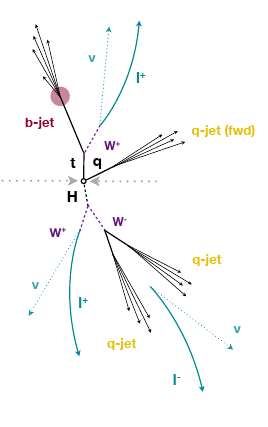
\includegraphics[scale=1.3]{Chapter1/jet.png}
		\caption[Topology of $tH$]{Topology of $tH$ process which generates two same sign muons, a forward jet and a b-jet.} 
		\label{jet}
	\end{figure}
%Quarks and gluons only exist in bound states. Because of it, we cannot isolate quarks except the top quark because of their decay times that don't form a bound state. When two quarks are separated, the strong force interacting between them increases. The energy transforms into quark anti-quark pairs. The hadronization results in a jet of particles. 
\begin{table}[ht]
	\caption[Expected number of events for $tH$ decay chain with 35.9 fb$^{-1}$ of integrated luminosity at center of mass energy of $\sqrt{s}$=13 TeV ]{Expected number of events for different $tH$ decay chains assuming integrated luminosity of 35.9 fb$^{-1}$. $l$ represents $\mu^{\pm},e^\pm, \tau^\pm$.}
	\begin{tabular}{|l|c|c|}
		\hline
		Decay chain & BR & Events\\
		\hline 
		\small{$tH \rightarrow$ $W^+bW^+ W^-$ $\rightarrow$ $\mu^+$ $\nu_\mu b$ $\mu^+\nu_\mu$ $q \bar{q}'$ } &\small{2.096 $\times$10$^{-3}$} & 1.173 \\
		\hline
		\small{$tH \rightarrow W$$^+ b$$W^+$ $W^-$ $\rightarrow$ $\mu^+\nu_\mu b$ $\mu^+\nu_\mu$ $l^- \bar{\nu_l}$ } &\small{3.37 $\times$ 10$^{-4}$} &0.899 \\
		\hline
		\small{$tH \rightarrow$ $W^+ b$ $\tau^+ \tau^-$ $\rightarrow$ $\mu^+ \nu_\mu b$ $ \mu^+ \nu_\mu \bar{\nu_\tau} l^-\bar{\nu_l} \nu_\tau$} &\small{3.637$\times$10$^{-4}$}&0.203 \\
		\hline
		\small{$tH \rightarrow$ $W^+ b$ $W^+ W^-$ $\rightarrow$ $\tau^+ \bar{\nu_\tau}b$ $\mu^+ \nu_\mu$ $q\bar{q}$ $\rightarrow$ $\mu^+ \nu_\mu$ $\bar{\nu_\tau}$ $\bar{\nu_\tau} b\mu^+ \nu_\mu$ $q \bar{q}$} &\small{1.890$\times$10$^{-4}$}&0.105 \\
		\hline
		\small{$tH \rightarrow W^+ b \tau^+ \tau^-$ $\rightarrow$ $\mu^+$ $\nu_\mu b$ $\nu_\tau$ $\mu^+$ $\nu_\mu \bar{\nu_\tau}$} $q \bar{q}$ &
		\small{1.681 $\times$10$^{-4}$} & 0.094 \\
		\hline
		\small{$tH \rightarrow W^+ b$ $W^+ W^-$ $\rightarrow$ $\tau^+ \bar{\nu_\tau} b \mu^+ \nu_\mu l^- \bar{\nu_l}$ $\rightarrow$ $\mu^+\nu_\mu$ $ \bar{\nu_\tau} \bar{\nu_\tau} b \mu^+ \nu_\mu l^- \bar{\nu_l}$} &\small{3.045$\times$10$^{-5}$}& 0.017\\
		\hline
		\small{$tH \rightarrow W^+ bZZ$ $\rightarrow$ $q \bar{q} bZZ$ $\rightarrow$ $q \bar{q} b \mu^+ \mu^- \mu^+ \mu^-$} & \small{1.966$\times$10$^{-5}$} &0.011\\
		\hline 
		\small{$tH \rightarrow$ $W^+ b$ $\tau^+ \tau^-$ $\rightarrow$ $\tau^+ \bar{\nu_\tau}b$ $\mu^+ \nu_\mu \bar{\nu_\tau} $ $q\bar{q}' \nu_\tau$ $\rightarrow$ $\mu^+ \nu_\mu \bar{\nu_\tau}\bar{\nu_\tau} b \mu^+ \nu_\mu \bar{\nu_\tau} $ $q\bar{q}' \nu_\tau$ } &\small{1.549 $\times$10$^{-5}$} & 0.008 \\
		\hline
	\end{tabular}
	\label{tdecay}
\end{table}

\pagebreak


\section{Backgrounds}
Several processes contribute to the background in this search:
\begin{itemize}
		\item $\bm{t\bar{t}W^{\pm}}$ and $\bm{t\bar{t}Z}$ $\bm{(t\bar{t}V)}$: One muon comes from a top and the other comes from the vector boson.
			\item $\bm{W^{+}Z}$: Diboson production with leptonic decays. One muon comes from $W$ boson and the other from $Z$ boson.
		\item $\bm{W^{\pm}W^{\pm}}$:A pair of same sign $W$ bosons generate a muon each one.
		\item $\bm{tZq}$: Processes with single top quarks associated with a Z boson, where $Z\rightarrow \mu^+ \mu^-$, also contribute to the background.
	\item $\bm{t\bar{t}t\bar{t}}$:In these type of events, one $t$ decays to $Wb$ and $W$ decays to a muon. The second muon comes from the other top decay.
	%Backgrounds are estimated directly from simulated events$\%$ which are corrected for data/MC differences and $\%$ inefficiencies in the same way as signal events. 
		\item$\bm{W^{+}W^{-}Z}$, $\bm{ZZZ}$ and $\bm{W^{+}ZZ}$ ($\bm{VVV}$): The leptonic decays of the $W$ or $Z$ bosons generate at least two same sign muons.
	\item $\bm{tZW^{+}}$:One muon comes from the $Z$ while the other same sign muon can come from $t$ or $W$. 
	\item $\bm{ZZ}$: Each muon comes from $Z$ boson decays.
			\item $\bm{t\bar{t}H}$: This Higgs production mechanism is considered a background in this analysis. The muons in this case comes from one top and Higgs decays. 
	\item $\bm{Fakes}$:This background refers to events where two muons come from $b$ meson decays in jets.
\end{itemize}
Table \ref{back} shows the decay chains for the backgrounds. Due to small expected event yields, the processes $W^\pm$ $W^\pm$,$tZq$,$t\bar{t}t\bar{t}$, $VVV$, $tZW^+$ and $ZZ$ are grouped as one called Rares in the results below.


\begin{table}[ht]
	\caption{Main backgrounds and their same sign $\mu\mu$ decay process }
	\centering
	\begin{tabular}{|c|l|}
		\hline
		Background & Decay process \\
		\hline
		$t\bar{t}W$ &$t\bar{t}W$ $\rightarrow$ $W^+ b W^- \bar{b}$ $\mu^+\nu_\mu$ $\rightarrow$ $\mu^+ \nu_\mu b$ $\mu^- \bar{\nu_\mu} \bar{b}$ $\mu^+ \nu_\mu$\\
		\hline
		$t\bar{t} Z$ & $t\bar{t} Z$ $\rightarrow$ $W^+ b$ $W^-\bar{b} \mu^+ \mu^-$ $\rightarrow$ $\mu^+ \nu_\mu b$ $\mu^- \bar{\nu_\mu} \bar{b}\mu^+ \mu^-$ \\
	 \hline
 $W^+ Z$ &$W^+ Z \rightarrow$ $\mu^+ \nu_\mu \mu^+ \mu^-$ \\
		\hline 
		$W^\pm$ $W^\pm$ & $W^+W^+$ $\rightarrow$$\mu^+\nu_\mu$$\mu^+ {\nu_\mu}$ \\
		\hline 
		$tZq$ & $tZq$ $\rightarrow$ $W^+$ $ b\mu^+ \mu^- q$ $\rightarrow$$\mu^+ \nu_\mu b$ $\mu^+\mu^- q$ \\
		\hline 
		$t\bar{t}t\bar{t}$ &$t\bar{t}t\bar{t}$ $\rightarrow$ $W^+ b$ $W^- \bar{b}$ $W^+ b$ $W^- \bar{b}$ $\rightarrow$ $\mu^+ \nu_\mu b$ $\mu^- \bar{\nu_\mu} \bar{b}$ $\mu^+ \nu_\mu b$ $\mu^- \bar{\nu_\mu} \bar{b}$ \\
		\hline 
		$W^+ W^- Z$ & $W^+ W^-$ $Z \rightarrow$ $\mu^+ \nu_\mu$ $\mu^- \bar{\nu_\mu} \mu^+ \mu^-$\\
		\hline 
		$ZZZ$ & $ZZZ \rightarrow$ $\mu^+ \mu^-\mu^+ \mu^-l^+ l^-$ \\
		\hline 
		$W^+ZZ$ &$W^+ZZ$ $\rightarrow$ $\mu^+ \nu_\mu \mu^+ \mu^- l^+l^-$ \\
		\hline 
		$tZW^+$ & $tZW^+ \rightarrow$ $W^+b \mu^+ \mu^- \mu^+ \nu_\mu \rightarrow \mu^+ \nu_\mu b \mu^+ \mu^- \mu^+ \nu_\mu$\\
		\hline
		$ZZ$ & $ZZ\rightarrow$ $\mu^+ \mu^- \mu^+ \mu^-$ \\
		\hline
		$t\bar{t}H$	& $t\bar{t}H$ $\rightarrow W^+b W^- \bar{b} W^+W^-$ $\rightarrow$ $\mu^+ \nu_\mu b$$\mu^- \bar{\nu_\mu}\bar{b}$ $\mu^+\nu_\mu$ $\mu^-\bar{\nu_\mu}$\\
		\hline 
	\end{tabular}
	\label{back}
\end{table} 

%Due to a large cross section, the main
%background contribution comes from WZ production.

\section{Event Selection}
In order to detect signal events and reject background, the following selections are applied, according to the CMS publication\cite{th1} 
\begin{itemize}
	\item The events must contain two muons with the same sign.
	\item Transverse momentum $p_{t}$ > 25 GeV for the highest $p_t$ muon and $p_{t}$ > 15 GeV for the lowest $p_t$ muon.
	\item A forward jet with $p_t$ > 40 GeV and $|\eta|$ > 2.4
	\item One or more b-tagged jets with $|\eta|$ < 2.4
\end{itemize}
%Also it is possible to obtain a study of three leptons, given the mentioned decays can produce them. 
The number of expected events after the event selection predicted by the Monte Carlo simulations used in the CMS publication are shown in Table \ref{tth-table} which corresponds to a integrated luminosity of 35.9 fb$^{-1}$\cite{th1}.
The backgrounds with the most events are $t\bar{t} W^\pm$, $t\bar{t}Z$ and Fakes. For the SM signal $tH$, the number of expected events is 2.14, while for the inverted coupling scenario ($k_t=-1$) the cross section is enhanced by a factor of approximately 10. 
These event yields will be used to estimate the signal sensitivity. The yields include statistical uncertainties due to the  Monte Carlo (MC) samples and systematic uncertainties as described in Table \ref{tth-table}. 

\begin{table}[ht]
	\centering
	\caption[Event yields for signal and backgrounds after the event selection]{Event yields for signal and backgrounds after the event selection for a integrated luminosity of 35.9 fb$^{-1}$. The uncertainties of yields include statistical and systematic\cite{th1}}
	\begin{tabular}{cc}
		\hline
		Process & Number of events \\
		\hline
		$t\bar{t}W$ & 68 $\pm$ 10 \\
		$t\bar{t}Z$ & 25.9 $\pm$ 3.9\\
		$WZ$ & 15.1$\pm$7.7\\
		Rares & 20.9 $\pm$ 4.9\\
		Fakes & 80.9 $\pm$9.4\\
		$t\bar{t}H$ & 24.2 $\pm$ 2.1 \\
		\hline
		$tH$ (SM) & 2.14 $\pm$ 0.13\\
		$tH$ ($k_t=-1$) &26.2 $\pm$ 2.2
	\end{tabular}	
	\label{tth-table}
\end{table}

\pagebreak

\section{Systematic uncertanties}
The uncertainties of the yields shown in Table \ref{tth-table} include systematic uncertainties due to the following sources, described in the CMS publication\cite{th1} and summarized here:
\begin{itemize}
\item The uncertainties on $t\bar{t}W$ and $t\bar{t}Z$ event yields are mainly due to the uncertainties of their production cross sections. 
\item The uncertainty on $WZ$ background is estimated using real data events in a three lepton control region. 
\item In the Rare background, a $50\%$ of uncertainty is assigned.
\item The uncertainty on the Fakes background is estimated using real data in a control region, defined by the muon identification criteria. 
\item For the Higgs processes $tH$ and $ttH$, the uncertainty are due to the theoretical parameters (e.g. the strong coupling constant $\alpha_s$ and Parton Distribution Functions (PDF) ) used in that simulation.
\end{itemize}

%control region: event selection with 3 leptons for compare simulation with real data. yield difference in that region is 50. Is taken and for wz is 50
%selection that allows to isolate a background respect to other backgrounds, that background allows to compare with real data 


\pagebreak
%The fake rate corresponds to non-prompt leptons.% Non prompt leptons are leptons that passed the selection, and usually comes from decays from b-jets (hadronized quarks). But due to jet signature is reconstructed as leptons, some particular signatures or errors in reconstruction, passed as leptons and then they called fakes leptons. Rare SM is a group of other processes: t$\bar{t}$t$\bar{t}$,WWW,WWZ,WZZ,WW,$t$Zq. Due to low number of events, they grouped the events as one histogram. 
\section{Multivariable discriminant}
Due to small signal to background ratio caused by the small cross section of $tH$, a multivariable discriminant, which separates signal from backgrounds, is necessary to optimize the signal sensitivity. The multivariable discriminant is a Boosted Decision Tree (BDT) that takes a set of input features and splits input data recursively based on those features\cite{tmva}. The features can be a mix of categorical and continuous data.
The BDT training is performed using several event variables.
In this analysis, the BDT discriminant was trained to discriminate against $t\bar{t}V$ background, because this background is one of the largest backgrounds. The variables used for the BDT were the following:

\begin{itemize}
\item Number of jets with $p_t$ > 25 GeV, $|\eta|$ < 2.4
\item Maximum $|\eta|$ of forward jet
\item Sum of lepton charges
\item Number of jets with $|\eta|$ > 1.0
\item $\Delta\eta$ between forward jet and b-jet with highest $p_t$
\item $\Delta\eta$ between forward jet and b-jet with lower $p_t$
\item $\Delta\eta$ between forward jet and closest muon
\item $\Delta\phi$ of highest $p_t$ same-sign muon pair
\item min $\Delta$R (muon pairs)\footnote{$\Delta R = \sqrt{ \Delta\eta^2 + \Delta\phi^2}$, where $\Delta R$ is the distance in the $\eta \phi$ plane}
\item $p_t$ of muon with lower momentum
\end{itemize}

Figure \ref{bdt2} shows the BDT distribution for signal and backgrounds.
\pagebreak
%Closure: hay jets en los eventos de tt (gluon-gluon -> tt + gluon ) que se pasan como muones. jet -> muon = fake

%Fakes: proceso de QCD que genera muchos jets (por ejemplo gluon-gluon -> gluons, quarks) : jet -> muons fakes are estimated data 

%bdt trained with fakes is not possible, due no simulation with that process 


\begin{figure}[ht]
	\centering
	\begin{minipage}[b]{0.6\textwidth}
		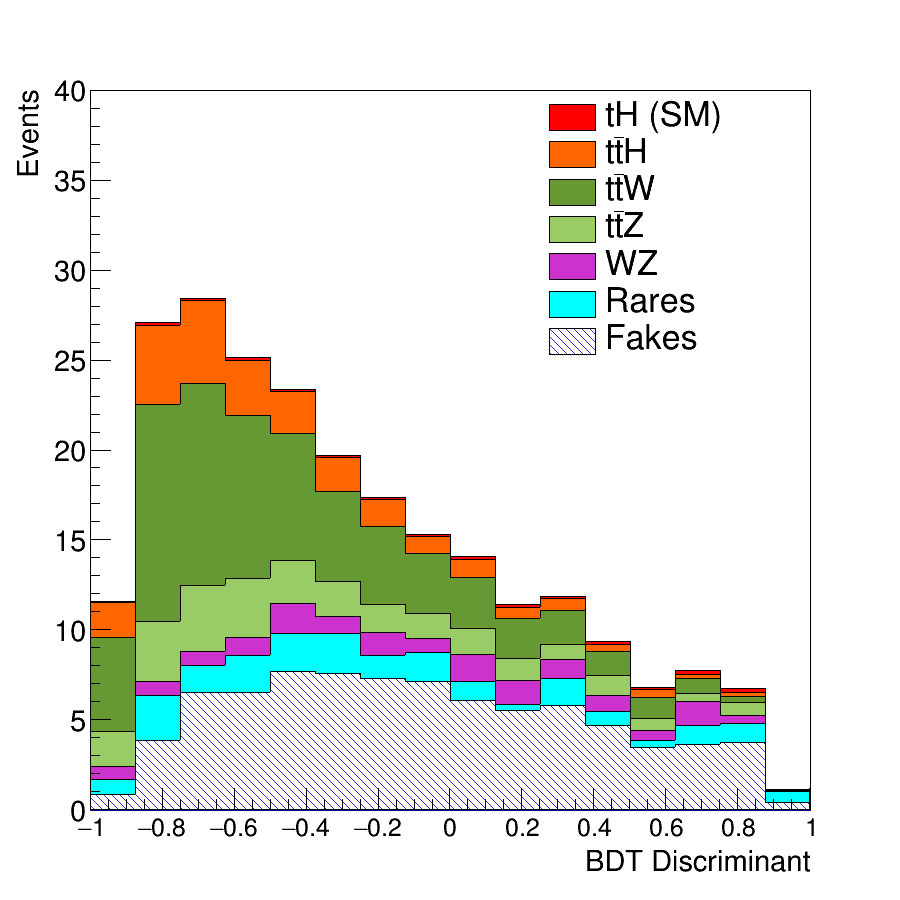
\includegraphics[width=\textwidth]{Chapter3/kos.png}
	\end{minipage}
	\hfill
	\begin{minipage}[b]{0.6\textwidth}
		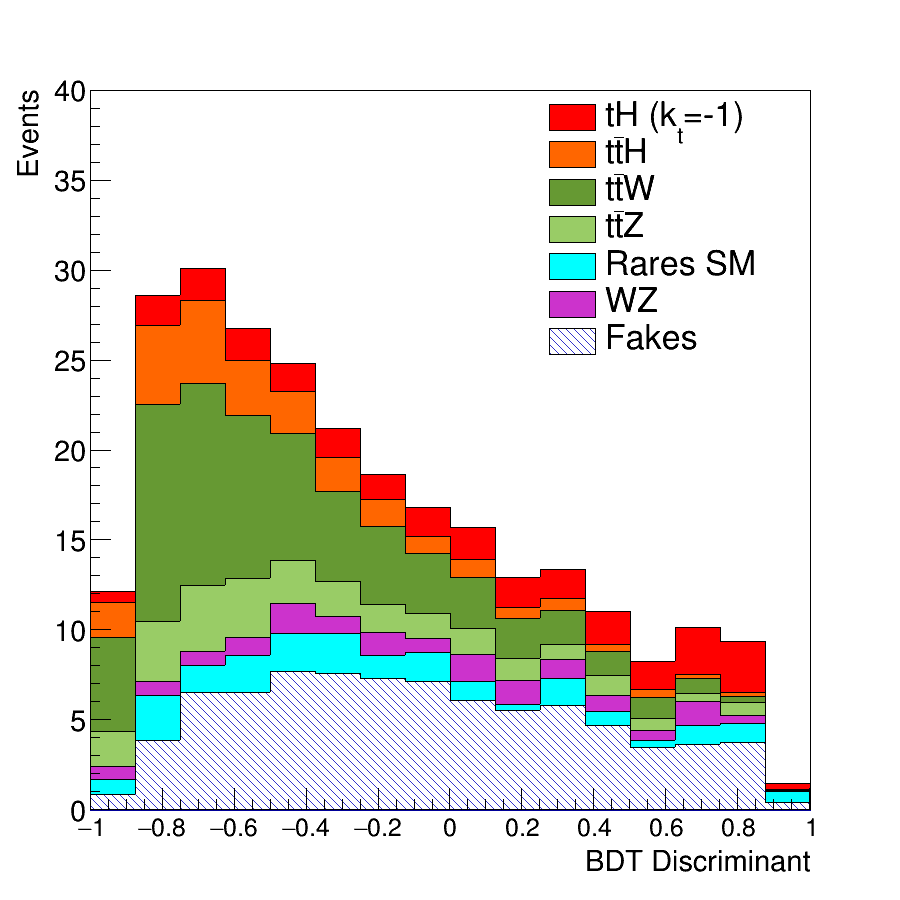
\includegraphics[width=\textwidth]{Chapter3/kos2.png}
	\end{minipage}
\caption[Distribution of BDT for signal and backgrounds ]{Distribution of BDT discriminant for signal and background in the case of SM (Up) and inverted coupling scenario (Down) \cite{th1}}
\label{bdt2}
\end{figure}

